\graphicspath{{members/paz/figures/}}

\subsection{Summary of Modeler View}\label{subsec:summary-of-modeler-view}
\input{members/paz/authors}

This discussion can be summarized into the following points as input to the
design process:

\begin{enumerate}
    \item The used models focus primarly on estimating yield using only visual information and a stable environmental setting.
    
    \item Each plant being analysed is set constrained to be at a set position with a fixed camera angle to take the pictures. The illumination is constrained by the greenhouse properties and a time given for the data acquisition. So invariance to camera pose and illumination are not required.
    
    \item The appearance of the object in the image is unconstrained. Invariance to the photometric properties of the plant is a requirement.
    
    \item The Leaf area can be recognized through the green color that is distinguishable from the surrounding ground color. Healthy leaves also appear in a  different green tone then unhealthy or dead leaves. These informations can be used for the design of a model-based approach.
    
    \item Information on exact values (green color treshhold, leaf level distance) can be refined via data-driven learning approaches.
    
\end{enumerate}

\subsection{Requirements to Modules Choices}
\input{members/paz/authors.tex}

\subsubsection*{Component selection}

The requirements to module choices motivate the use of model-based and data-driven components. In this implementation of the project the focus lies on model based component choices. In the following we enumerate the link between module choices and model.

\begin{enumerate}
    \item \textbf{Constrained information Input:} Due to the fact that the amount of information gathered is limited to visual information, the chosen modules need to estimate the wanted information as accurate as possible. We chose the LAI (Leaf area index) as the parameter due to the strong correlation to yield \cite{heuvelink2004effect} and the possibility to gather this parameter using image processing.

    \item \textbf{Mensuration exploits contextual priors:} The mensuration module can exploit the greenhouse setting in the acquisition setup, i.e. the cameras are set at a fixed angle and distance from the plant. We know information about the height of the camera and the center point. The intrinsic camera calibration is assumed to be known.

    \item \textbf{Optimizing defect detection:} The Image segmentation model is set up to be variable and adjustable to different tones of green. This enables the module to adjust to changes in the leaf color and detect sick or dead leaf structure. The segmentation is deviced to be able to match different lighting situations and plant defects by adjusting the green threshold.

    \item \textbf{Scalability, Extensibility of modules to Novel Settings:} The strong modulation of the application allows the option to split, rearrange and reuse specific modules in novel settings.
\end{enumerate}

\subsection{Discussion on Strengths/Limitations of the Leaf Area Index model}
\input{members/paz/authors.tex}

As mentioned above the LAI gives us a good representation of the PAR (photosynthetically active radiation) which highly influences biomass as well as yield production. \cite{hossain2017leaf} The yield predicted using the above mentioned modules is  useful when the plant is in a full grown state before starting to produce yield. We are able to estimate yield using the LAI at the moment of time the image is taken. Yield predicitons made by this application are used to estimate yield in the near future. In addition the approximation for full grown tomato plants is robust to inaccuracies. This is explained by the saturation of radiation that can be absorbed.The intercepted light shows a saturation at a specific LAI value. Due to the nature of the project being autonomous to a certain degree the plants do not get unnecessary leaves removed and these leaves are included in the estimated LAI. So the correlation between the LAI and the intercepted light is represented in a flattening curve. See in \ref{fig:LaiCurve}\\

\begin{figure}[H]
    \centering
    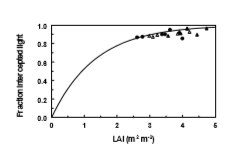
\includegraphics[scale=1.2]{LAI.PNG}
    \caption{\textit{Note: Measurements from \cite{heuvelink2004effect} showing the Fraction intercepted light as function of measured leaf area index (LAI), determined once per month starting from mid-March until mid-August for three leaf picking strategies: reference, high and maximum LAI.  Curve equation: fract. intercept. = 1-e-0.75 LAI.  Each data point based on 3 plots}}
    \label{fig:LaiCurve}
\end{figure}

Under following conditions the method would fail:

\begin{enumerate}
    \item When the plant doesn't grow in the intended position it is not possible to estimate the accurate height of the plant and the canopy size and plant height will be esimated with false values. A tilt correction is included in the edge detector to fix minor tilt angles, but it fails once the this angle reaches a certain treshhold. The module will follow wrong assumptions to predict the leaf area and will not be able to give an accurate estimation of future yield.

    \item If the plant shows some abnormalities to the assumed norm. If the leaf density is abnormal low or high in any level of the plant the approximated yield will deviate from the intended value.

    \item Different morphology can not be recognized by the system and will be treated as the assumed cone shaped plant structure.
\end{enumerate}
